% Данный файл распространяетсяя под лицензией CC BY 4.0. Текст лицензии размещён на https://creativecommons.org/licenses/by/4.0/
% (c) Кафедра системного программирования, 2025

\documentclass[a4paper]{article}

\usepackage[a4paper, top=8mm, bottom=8mm, left=8mm, right=8mm]{geometry}

\usepackage{polyglossia}
\setdefaultlanguage[babelshorthands=true]{russian}
\setotherlanguage{english}

\usepackage{fontspec}
\setmainfont{FreeSerif}
\newfontfamily{\russianfonttt}[Scale=0.7]{DejaVuSansMono}

\usepackage[tiny, compact]{titlesec}

\usepackage{titling}
\setlength{\droptitle}{-1cm}
\pretitle{\begin{center}\begin{bfseries}\Large}
\posttitle{\par\end{bfseries}\end{center}}
\preauthor{\begin{center}\normalsize}
\postauthor{\par\end{center}\vspace{-1.8cm}}

\usepackage{hyperref}
\usepackage{bookmark}
\usepackage{csquotes}
\usepackage{graphicx}

\title{Разработка Python-обёртки для библиотеки Spla с подготовкой к публикации на PyPI}

\author{Смирнов Антон Игоревич}

\date{}

\begin{document}

\maketitle

\begin{flushright}
    Группа: \emph{2025.M71-мм}

    Кафедра: \emph{кафедра системного программирования}

    Научный руководитель: \emph{Григорьев Семён Вячеславович,}\\
    \emph{доцент кафедры системного программирования,}\\
    \emph{кандидат физико-математических наук}

    Номер семестра практики: \emph{2}
\end{flushright}

\section{Постановка задачи}

Библиотека Spla \cite{spla} предоставляет инструменты для работы с разреженными матрицами и векторами с ускорением на GPU через OpenCL. Основная C++ часть библиотеки полностью работоспособна, Python-обёртка существует, но не готова к полноценному распространению: отсутствует автоматизированная сборка, нет тестов и не настроена публикация на PyPI.

\textbf{Целью работы является} подготовка Python-обёртки библиотеки Spla к публикации: разработка тестов, проверка работы на целевой платформе и настройка автоматической публикации через GitHub Actions.

Результаты работы необходимы для упрощения установки библиотеки конечными пользователями и обеспечения автоматической проверки её работоспособности. В выполнении работы заинтересованы разработчики библиотеки Spla и её потенциальные пользователи.

В рамках работы были поставлены и решены следующие задачи:
\begin{enumerate}
    \item Собрать C++ библиотеку Spla под Windows (получить \texttt{spla\_x64.dll}).
    \item Разработать модульные тесты для \texttt{Vector}, \texttt{Matrix}, \texttt{Scalar}, \texttt{Array}, \texttt{Op}.
    \item Создать структуру тестовых данных (\texttt{tests/data/}).
    \item Настроить автоматическую публикацию на PyPI через GitHub Actions.
    \item Проверить работоспособность обёртки на Windows с GPU Intel Arc.
\end{enumerate}

\section{Описание предлагаемого решения}

Архитектура Python-пакета \texttt{pyspla} показана на рисунке \ref{fig:uml}.

\begin{figure}[ht]
    \centering
    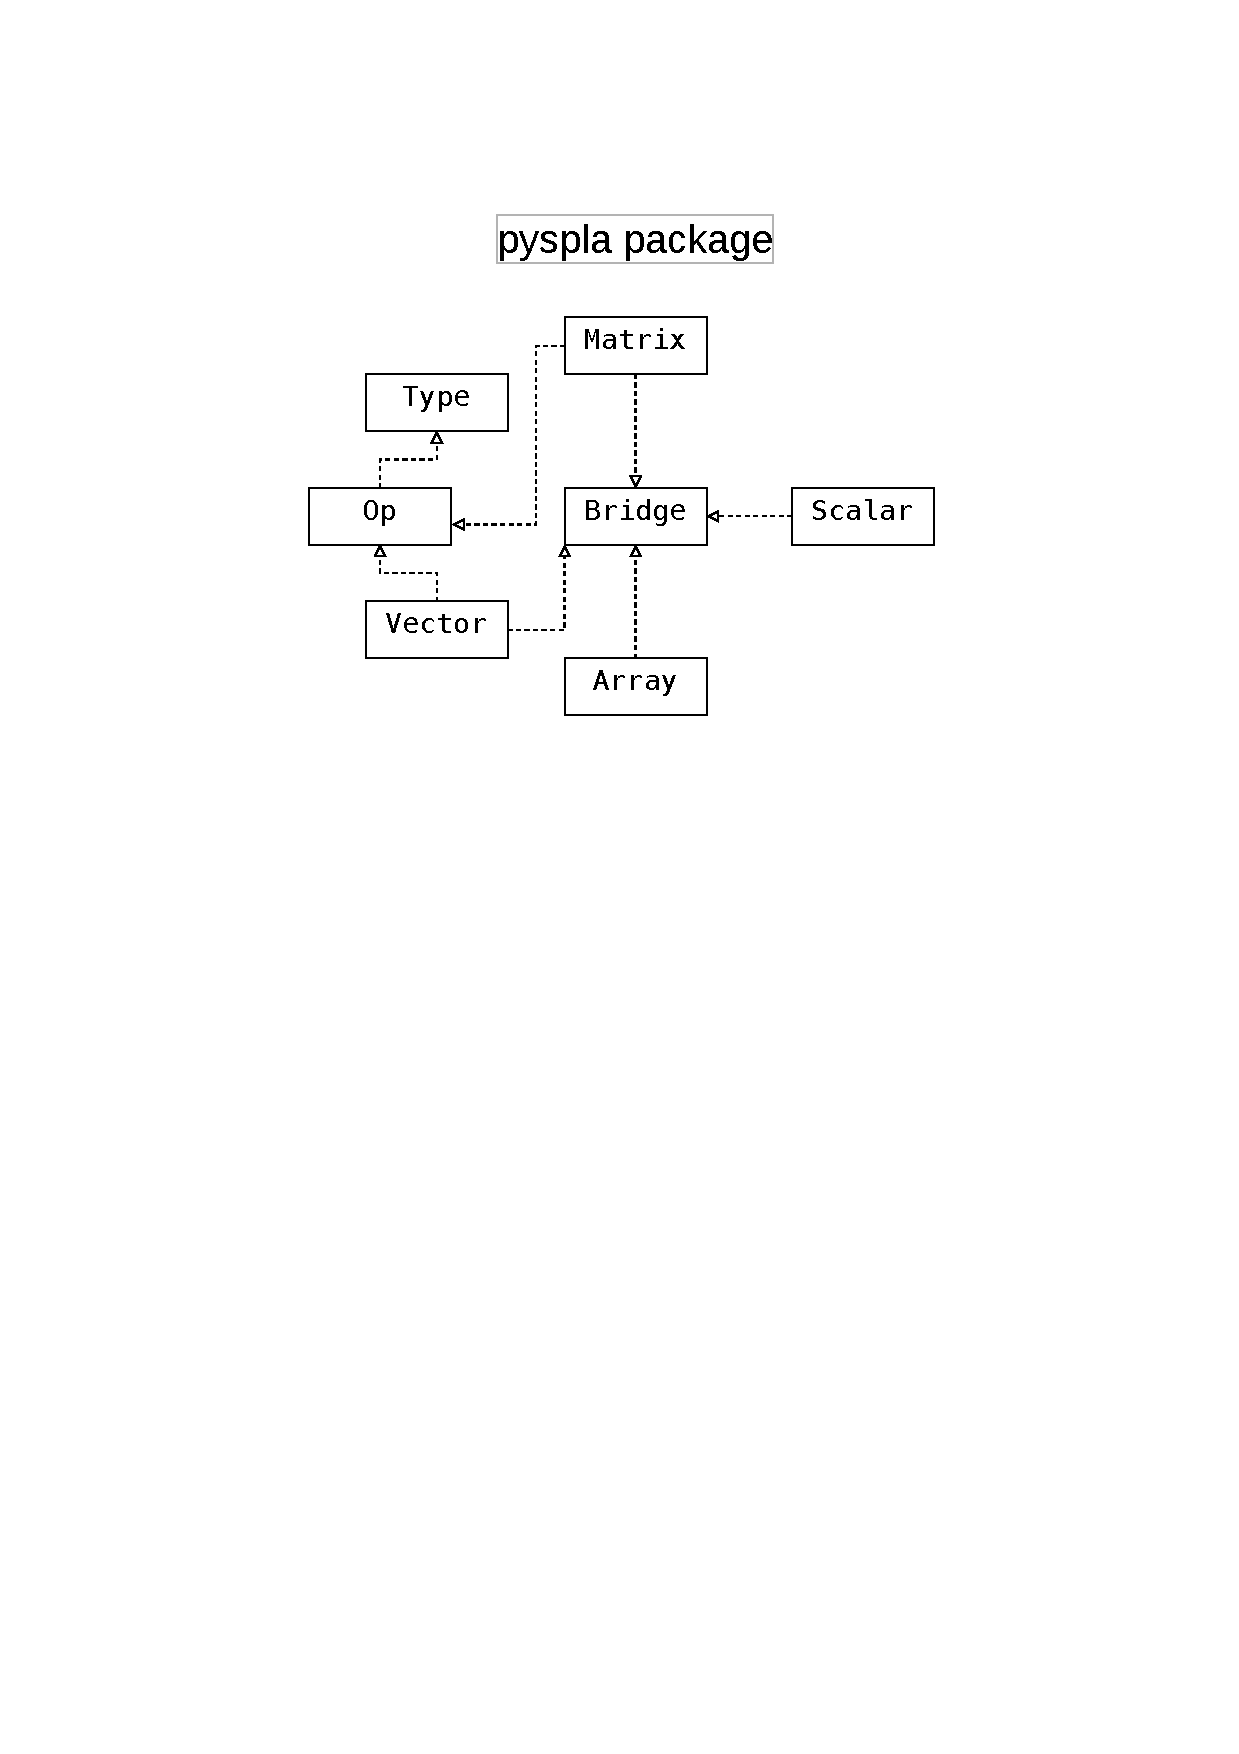
\includegraphics[width=0.7\textwidth]{images/pyspla_architecture.pdf}
    \caption{Архитектура Python-пакета pyspla}
    \label{fig:uml}
\end{figure}

Ключевые компоненты пакета:
\begin{itemize}
    \item \texttt{Bridge}~--- загрузка C++ библиотеки и взаимодействие с ней.
    \item \texttt{Matrix}, \texttt{Vector}, \texttt{Scalar}, \texttt{Array}~--- основные классы для работы с данными.
    \item \texttt{Op}~--- унарные и бинарные операции.
    \item \texttt{Type}~--- типы данных (INT, FLOAT, BOOL).
\end{itemize}

\textbf{Сборка C++ библиотеки.} Сборка выполнена с использованием Visual Studio 2026 и CMake. После сборки \texttt{spla\_x64.dll} скопирована в \texttt{python/pyspla/} для доступа из Python.

\textbf{Модульное тестирование.} Тесты написаны с использованием \texttt{unittest} и покрывают основные классы обёртки: \texttt{Vector}, \texttt{Matrix}, \texttt{Scalar}, \texttt{Array}, \texttt{Op}. Тесты используют параметризованные данные из \texttt{tests/data/}.

\textbf{Автоматизация публикации.} Добавлен GitHub Actions workflow, который активируется при создании тега вида \texttt{v0.0.6}, собирает пакет и публикует его на PyPI.

Реализация осуществлялась с использованием Python, C++17, OpenCL, CMake и GitHub Actions.

\section{Эксперименты}

Проверка корректности работы включала:
\begin{itemize}
    \item Сборку Python-пакета командой \texttt{python -m build}.
    \item Запуск модульных тестов.
    \item Проверку работоспособности на целевой платформе.
\end{itemize}

\textbf{Среда:} Windows 11, Intel Core i7, Intel Arc Graphics (OpenCL 3.0), Python 3.14, MSVC 19.50, CMake 3.x.

Запущено 16 модульных тестов, все успешно пройдены. Пример вывода для сложения векторов:
\begin{verbatim}
a: [5, 0, 10, 15, 0]
b: [0, 3, 7, 0, 2]
expected: [5, 3, 17, 15, 2]
result: [5, 3, 17, 15, 2]
\end{verbatim}

В процессе тестирования обнаружена ошибка в \texttt{scalar.py}: оператор вычитания выполнял сложение. Ошибка была исправлена, корректность исправления подтверждена тестами. Исправление включено в подготовленный Pull Request №239 в основной репозиторий проекта.

GitHub Actions workflow для публикации настроен корректно и ожидает создания тега. Проверены корректность сборки пакета и выполнение workflow до этапа публикации. Для фактической публикации требуется создание релизного тега и наличие учётных данных PyPI.

\section{Заключение}

В ходе выполнения работы получены следующие результаты:

\begin{itemize}
    \item Разработаны модульные тесты для всех ключевых компонентов обёртки (Vector, Matrix, Scalar, Array, Op). Все 16 тестов проходят.
    \item Добавлен GitHub Actions workflow для автоматической публикации на PyPI при создании тегов.
    \item Обнаружена и исправлена ошибка в операторе вычитания класса \texttt{Scalar}.
    \item Подготовлена структура тестовых данных для параметризованного тестирования.
\end{itemize}

Репозиторий с реализацией: \url{https://github.com/LuhTonkaYeat/spla}

Pull Request в основной репозиторий: \url{https://github.com/SparseLinearAlgebra/spla/pull/239}

Решение находится на ревью в основном репозитории проекта.

\begin{thebibliography}{9}
\bibitem{spla}
Исходный код библиотеки Spla. URL: \url{https://github.com/SparseLinearAlgebra/spla}
\end{thebibliography}

\end{document}